\chapter{Introduction}

\dictum[Теодо́сій Григо́рович Добжа́нський (Theodosius
Dobzhansky)\footnotemark]{Nothing in biology makes sense […]}
\footnotetext{\citet{Dobzhansky:1973}}

\section{The central dogma}

% <<<
At the core of every living being is its genetic inheritance. The genetic
inheritance is what is being passed down from parents to their offspring, and
contains a blueprint detailing how to construct a new individual from a single
cell in a process called \define{embryogenesis}. This genetic inheritance is
physically present in the form of \dna in almost every living cell.\footnote{And
to some extent in non-living particles called \define{viruses}.}

As a medium of information storage, \dna is complemented by two other types of
molecules in the cell that, respectively, carry out the instructions encoded in
the \dna by performing specific biochemical functions, and serve as an
intermediary between information storage and execution. The intermediaries,
which are called \define{\rna}, copy out specific parts of the complete
instructions from the \dna and carry them to factories which translate the
instructions into highly specialised machines. These machines are called
\define{proteins}. The \define{central dogma of molecular biology} states that
information is thus transmitted from \dna to \rna, and from \rna to proteins,
but never from proteins back to \rna or \dna (\cref{fig:central-dogma})
\citep{Crick:1958,Crick:1970}. When first published, the central dogma concisely
summarised the available evidence at the time. Now, more than half a century
later, this still largely holds true.

\textfig{central-dogma}{body}{0.75\textwidth}
    {The central dogma of molecular biology.}{The solid arrows represent
    observed transfers of information; the dashed arrows represent what
    \citet{Crick:1970} referred to as “potential” transfers; today we know that
    the transfer \(\text{\rna}\rightarrow\text{\dna}\) does in fact occur under
    certain circumstances; the transfer \(\text{\dna}\rightarrow\text{protein}\)
    has still not been observed. Notably, the \emph{absent} transfers in the
    original publication are still considered largely non-existent.}

The very high-level view of the central dogma was complemented by a detailed
mechanistic description over the years, and the efforts to fill in all the
details are still ongoing. In this thesis I will present the results of my
exploration of one minute aspect concerning the translation of \rna into
proteins. To better explain how it fits into the general picture of the central
dogma, we first need to understand its leading actors and their interplay. The
three main roles in the central dogma are fulfilled by \dna, \rna and proteins,
respectively, and we are now going to take a look at all of them in turn.
% >>>

\subsection{\abbr{dna}}

% <<<
\dna consists of a long chain of \define[{\defineword{nucleotide} molecule
consisting of a ribose, one or more phosphate groups and a nucleobase (example:
cytidine monophosphate, a nucleotide of cytosine)\footnotemark\\%
\marginfig{nucleotide}}]{nucleotides}\footnotetext{Figure adapted from
\url{https://commons.wikimedia.org/w/index.php?title=File:Nucleotides_1.svg&oldid=128814238}}.
The chemical structure of nucleotides enables them to polymerise into long,
relatively stable chains. \dna is made up of nucleotide monomers, consisting of
one or more phosphate groups coupled to a \define[\defineword{nucleoside}
nucleobase coupled to a ribose]{nucleoside}, each of which contains any of four
different types of \define{nucleobases}: adenine (\nA), cytosine (\nC), guanine
(\nG) and thymine (\nT). Thus, \dna can be thought of as a long string of four
different letters, and that is indeed how it is often represented. Text is
written from left to right in Western cultures. By convention, \dna is written
from \fivep to \threep. The numbers refer to the numbering of the carbon atoms
in each nucleotide’s ribose, with the \threep carbon atom forming a covalent
bond with the phosphate of the next nucleotide, which is itself attached to the
\fivep carbon of its ribose. In this way, a \fivep \ce C atom is exposed at one
end of the chain, and a \threep \ce C is exposed at the other.

\dna is present in the cell in the form of double-stranded helices: each \dna
molecule consists of two paired chains, wound tightly around each other, with
the bases on each chain pairing up such that every \nA on one chain is paired
with a \nT on the other, and each \nC is paired with a \nG. This striking
symmetry is known as Watson–Crick base pairing, after its discoverers
\citep{Watson:1953}. Thus, \dna is made up of two complementary strands,
redundantly holding the genetic information. This redundancy is used in \dna
copying (which occurs at every cell division, and is the mechanism by which
genetic information is passed from one cell to its offspring) to synthesise two
newly formed \dna molecules, of which each contains one strand of the parent
\dna molecule (\define{semiconservative replication}) \citep{Meselson:1958}.

\begin{figure}
    \hspace{-\dimexpr\oddsidemargin+1in}%
    \makebox[\textwidth][l]{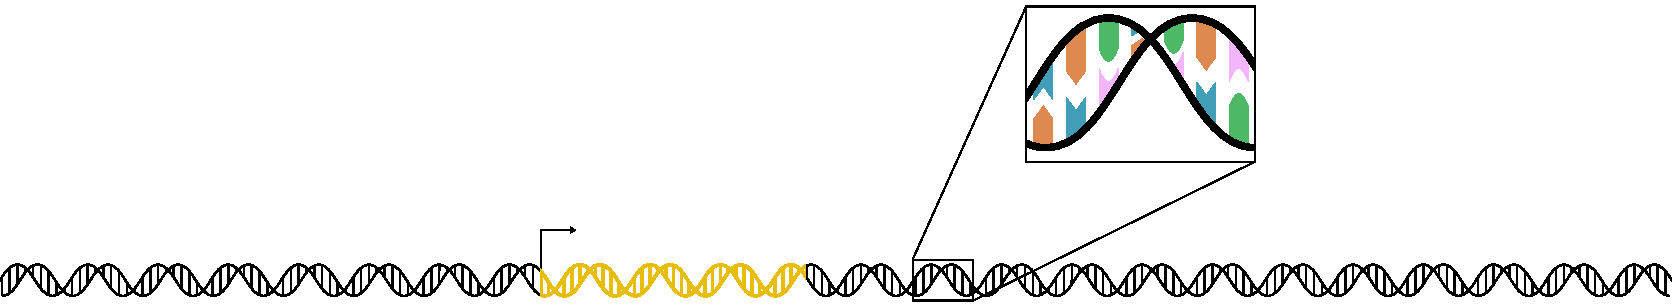
\includegraphics[width=\paperwidth]{dna-helix}}
    \figcap{dna}{\abbr{dna} double helix}{with a single, transcribed gene. The
    intertwined lines form the phosphoribose backbone of the \dna. Each vertical
    line connecting the backbones correspond to a nucleotide pair. The zoomed in
    cartoon shows the complementary base pairing. The length of the gene is
    understated, the overwhelming majority of transcribed pieces of \dna are
    much longer (protein-coding genes being many hundred to thousands of base
    pairs long).}
\end{figure}

\dna is not made up of a single polymer chain, but rather is partitioned into
several long pieces, called \define{chromosomes}. Each chromosome forms a single
molecule. However, even on each chromosome the genetic information is not stored
in one consecutive piece: Rather, \dna consists of relatively short stretches
encoding a specific function, separated by long stretches that do not directly
encode any function. The “function” is what is transmitted, as per the central
dogma, to \rna and, in many cases, on to proteins. Such self-contained,
functional stretches are called \define[\defineword{gene} self-contained stretch
of \abbr{dna} that is transcribed to perform a function]{genes}. To perform its
function, a gene has to be transcribed into a catalytically active form, the
\rna.
% >>>

\subsection{\abbr{rna}}

% <<<
\rna is the product of transcription of a gene from \dna. Unlike the latter,
\rna is created as a single strand. This has two consequences: First, \rna is
much less stable than \dna, and slowly degrades. \rna thus has a finite
life-time, and the pool of \rna must be replenished by continuous transcription.
Second, single-stranded ribonucleic acid spontaneously changes its spatial
conformation by forming Watson--Crick base pairs between nucleotides in its own
sequence, where this is \define[\defineword{steric effect} atoms occupy discrete
space and cannot overlap]{sterically} possible (i.e.\ where forming such a bond
does not require bending the chain too much to “snap” it). The resulting
structure can have functional consequences for the \rna. Because the structure
is determined by, and exists on a higher level than the sequence identity of the
\rna, it is called \define{secondary structure}.

Another difference between \dna and \rna is the use of slightly different
nucleobases: instead of \nT, \rna uses \nU (uracil), which, like \nT, base-pairs
with \nA. Despite the fact that the genetic information is encoded in virtually
the same way in \dna and \rna, transcription of \dna into \rna requires a
complex machinery. The core of this machinery is a complex enzyme called an
\define{\rna polymerase}. In eukaryotes, three different, evolutionarily related
\rna polymerases (\pol1, \pol2 and \pol3) are responsible for transcribing
different types of \rna.

\rna performs numerous different functions, but one very important subcategory
of \rna does not perform any function on its own; rather, it is an intermediary
between the genetic information on the \dna and the final protein product, which
in turn performs cellular functions. This class of \rna is called \mrna.
\mrna[s] are the product of the transcription of protein-coding genes by \pol2.
By contrast, \rna[s] which are not protein-coding are denoted as \ncrna.
Transcription of \mrna requires an exquisite control, and many different \tf[s]
are known to regulate the activity of transcription of different genes in
different cellular conditions.

This results in different \mrna genes being transcribed at highly different
levels, leading to several orders of magnitude of difference in \mrna abundance.
Even more strikingly, the same \mrna can be transcribed at different levels
under different conditions. \mrna is further processed in several steps before
the mature \mrna is exported from the cell’s nucleus into the cytoplasm, where
it is translated into proteins, and, over time, decays. Taken together, this
leads to very differentiated \mrna profiles under different conditions, which
imbue the cells with a unique phenotype. This forms the basis of cellular
differentiation into different cell types and tissues in multicellular
eukaryotes.
% >>>

\subsection{Proteins}

% <<<
Proteins, finally, are the main effectors of cell function. Like \dna and \rna,
they consist of chains of smaller molecules, so-called
\define[{\defineword{amino acid} molecule consisting of an amino–carboxyl
backbone and a specific side-chain (example: valine)\\%
\marginfig{amino-acid}}]{amino acids}, which are strung together to form
\define{polypeptides}. Each amino acid is a small molecule with unique
properties which, jointly, shape the function of the final protein. Individual
amino acids are strung together in a chemical reaction that links a carboxyl
group covalently with an amino group on the next amino acid to form a
\define[\defineword{peptide bond} a covalent bond formed between a carboxyl and
an amino group: \ce{COOH + NH2 -> CO-NH + H2O}]{peptide bond}
\citep{Alberts:2002}. Polypeptides, like many \rna[s], form secondary structures
via non-covalent bonds between amino acids, which are a function of the amino
acid sequence. Beyond this, proteins form even higher order three-dimensional
conformations called tertiary structures. When multiple proteins aggregate into
a complex consisting of several subunits, we speak of quarternary structure.

All these different levels of spatial organisation of proteins lead to the
creation of highly complex structures from originally one-dimensional chains. It
is their intricate structure which allows them to perform precise tasks in the
cell. Because they are the work horses of the cells, proteins are highly
abundant, with some proteins being present million-fold at any given moment
\citep{Milo:2013}. This is only possible because a single gene is transcribed
multiple times at once, and each resulting \mrna can be translated several
times, and simultaneously, before being degraded. The path
\(\text{\dna}\rightarrow\text{\rna}\rightarrow\text{protein}\) thus facilitates
an amplification from a single gene copy to many orders of magnitudes more
copies of the resulting protein. Despite the fact that multiple protein copies
can be created from a single \mrna molecule, and that the number varies from
transcript to transcript, protein abundance is predominantly determined by the
abundance of \mrna[s] \citep{Li:2014,Jovanovic:2015,Csardi:2014}.
% >>>

\section{Transcription \& translation}

\subsection{Transcription}
\label{sec:transcription}

% <<<
As mentioned, three different polymerases are responsible for transcribing genes
encoded in the \dna into different types of \rna. The precise ways in which the
different polymerases transcribe genes into their \rna products differ but the
fundamental aspects of transcription are similar. In all cases, a
\define[\defineword{motif} pattern describing a family of short sequences which,
though variable, have some degree of similarity]{motif} in the \dna sequence
initiates binding of a number of \tf proteins to the \dna. Such motifs, called
\define{promoters}, are found in the immediate vicinity of the \tss of their
target genes --- either upstream of the \tss or following closely after it,
inside the gene body. Once the \tf[s] have bound to the \dna on top of the \tss,
a polymerase attaches to the \dna and is held in place by the \tf[s].
Subsequently, the polymerase pries the double strand apart and starts
synthesising a new strand of \rna which pairs complementary with one of the
strands on the \dna (the \define{template strand}). The new \rna[’s] sequence is
thus identical to the other \dna strand (the \define{coding strand}). The \rna
is produced in the direction \fivep--\threep, implying that the template strand
is read in the direction \threep--\fivep during transcription. Once the first
few nucleotides of the \rna have been synthesised, the polymerase disassociates
from the \tf proteins, and the polymerase starts moving along the gene body,
transcribing it as it goes (this may require the presence of other \tf[s] called
\define{activators}, which are recruited by \define{enhancer} motifs elsewhere
on the \dna).

Eukaryotic chromosomes are very long — human chromosome \num{1} is around
\SI{8.5}{\centi\metre} stretched from end to end — and, to fit into the cell, is
tightly packed into a space-efficient conformation. To achieve this, \dna is
coiled around \define{histones}, small protein complexes, to form
\define[\defineword{nucleosome} complex of \dna wrapped around an ensemble of
eight core histones]{nucleosomes}. Too tight packing, however, has the
side-effect of making the \dna inaccessible to the transcription machinery. It
is thus a common feature of gene regulation to control the chromatin structure,
and thus to control the accessibility of the \dna for \tf[s] and the
polymerases. Furthermore, histones can be marked in several ways — via addition
or removal of acetyl or methyl groups — which are recognised by \tf[s] and thus
once again either facilitate or inhibit transcription \citep{Alberts:2002}. In
addition to enhancers and promoters, chromatin structure and the modification of
histones thus regulate the activity of genes.

\todo[inline]{Figure: Transcription}
% >>>

\subsection{The genetic code}

% <<<
The process by which proteins are created from \mrna transcripts is more complex
than the 1:1 transcription of \dna into \rna, which after all use a common
alphabet to encode the information they carry. By contrast, the
\define{translation} of \mrna transcripts into proteins requires a code to
interpret the genetic information.

There are \num{20} different amino acids that are encoded by just \num{4}
different nucleotides. To allow this, several nucleotides must be combined to
form a larger unit coding for an amino acid. In the universal \define{genetic
code}, shared by all known species, this is accomplished by grouping three
consecutive nucleotides together to form non-overlapping \define{codons} along
the \mrna. This results in \(4^3 = 64\) possible codons, vastly more than there
are amino acids. As a consequence, the genetic code is \define{degenerate}: most
amino acids can be encoded by more than a single codon.

\begin{table}[!ht]
    \centering
    \def\s{\footnotesize stop}
    \def\h#1#2{\multicolumn{1}{#1}{\abbrsc{#2}}}
    \begin{tabu} to \textwidth {@{}
            >{\collectcell\codon}l<{\endcollectcell}
            >{\collectcell\anticodon}l<{\endcollectcell}
            l @{\qquad}
            >{\collectcell\codon}l<{\endcollectcell}
            >{\collectcell\anticodon}l<{\endcollectcell}
            l @{\qquad}
            >{\collectcell\codon}l<{\endcollectcell}
            >{\collectcell\anticodon}l<{\endcollectcell}
            l @{\qquad}
            >{\collectcell\codon}l<{\endcollectcell}
            >{\collectcell\anticodon}l<{\endcollectcell}
            l @{}}
        \toprule
        % Nasty, hand-coded length values.
        \noalign{\vskip-4pt}
        \h{@{}l}{C} & \h{l}{A} & \h{l}{AA} &
        \h{@{}l}{C} & \h{l}{A} & \h{l}{AA} &
        \h{@{}l}{C} & \h{l}{A} & \h{l}{AA} &
        \h{@{}l}{C} & \h{l}{A} & \h{l@{}}{AA} \\[-2pt]
        \midrule
        UUU & AAA & Phe & UCU & AGA & Ser & UAU & AUA & Tyr & UGU & ACA & Cys \\
        UUC & GAA & Phe & UCC & GGA & Ser & UAC & GUA & Tyr & UGC & GCA & Cys \\
        UUA & UAA & Leu & UCA & UGA & Ser & UAA & UUA & \s  & UGA & UCA & \s \\
        UUG & CAA & Leu & UCG & CGA & Ser & UAG & CUA & \s  & UGG & CCA & Trp \\
        \addlinespace
        CUU & AAG & Leu & CCU & AGG & Pro & CAU & AUG & His & CGU & ACG & Arg \\
        CUC & GAG & Leu & CCC & GGG & Pro & CAC & GUG & His & CGC & GCG & Arg \\
        CUA & UAG & Leu & CCA & UGG & Pro & CAA & UUG & Gln & CGA & UCG & Arg \\
        CUG & CAG & Leu & CCG & CGG & Pro & CAG & CUG & Gln & CGG & CCG & Arg \\
        \addlinespace
        AUU & AAU & Ile & ACU & AGU & Thr & AAU & AUU & Asn & AGU & ACU & Ser \\
        AUC & GAU & Ile & ACC & GGU & Thr & AAC & GUU & Asn & AGC & GCU & Ser \\
        AUA & UAU & Ile & ACA & UGU & Thr & AAA & UUU & Lys & AGA & UCU & Arg \\
        AUG & CAU & Met & ACG & CGU & Thr & AAG & CUU & Lys & AGG & CCU & Arg \\
        \addlinespace
        GUU & AAC & Val & GCU & AGC & Ala & GAU & AUC & Asp & GGU & ACC & Gly \\
        GUC & GAC & Val & GCC & GGC & Ala & GAC & GUC & Asp & GGC & GCC & Gly \\
        GUA & UAC & Val & GCA & UGC & Ala & GAA & UUC & Glu & GGA & UCC & Gly \\
        GUG & CAC & Val & GCG & CGC & Ala & GAG & CUC & Glu & GGG & CCC & Gly \\
        \bottomrule
    \end{tabu}
    \tabcap{genetic-code}{The genetic code.}
        {Shown is each codon (“\abbrsc{C}”), its potential corresponding
        anticodon (“\abbrsc{A}”) and the three-letter abbreviation of the
        corresponding amino acid (“\abbrsc{AA}”). \codon{AUG}, in addition to
        encoding methionine, also signals the start of translation. Not all
        anticodons exist in all species. Each anticodon is the reverse
        complement of its corresponding codon (adapted from
        \citet{Dos_Reis:2004}).}
\end{table}

Codons furthermore serve as control points by defining where the translated
sequence on the \mrna starts and ends. The codon \codon{AUG}, in addition to
encoding the amino acid methionine, also marks the start of the coding sequence.
Three codons do not encode any amino acid, and instead signal the stop of
translation (\codon{UAA}, \codon{UAG}, \codon{UGA}). As a consequence, every
coding sequence starts with \codon{AUG}, ends with one of the stop codons, and
has a length divisible by \num{3}. \Cref{tab:genetic-code} contains a tabular
representation of the genetic code, which is valid, with only minor variations,
for all three domains of life.

During translation, individual codons on the \mrna transcript are successively
paired up with their matching amino acid. However, unlike in translation, this
pairing does not happen automatically. It requires an intermediate adapter
molecule acting as an interface between the codon and the amino acid.
% >>>

\subsection{Transfer \abbr{rna}}

% <<<
Individual codons are translated into their corresponding amino acid with the
aid of adapter molecules carrying a specific amino acid, and which recognise the
matching codon. This codon recognition is possible because the adapter molecules
are themselves \abbr{rna}s, and the codon is matched via complementary base
pairing of a part of the \rna sequence termed the \define{anticodon}. These
adapter molecules are called \trna.

\trna[s]\marginpar{
    \vspace{-12ex}% Necessary to fix figure going over bottom of page.
    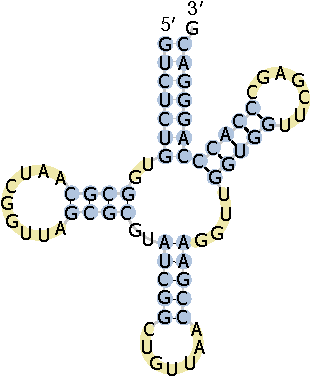
\includegraphics[width=\marginparwidth]{trna-asn}
    \vspace{-\baselineskip}
    \figcapof{trna-asn}{\xtrna{Asn} secondary structure.}{ The \abbr{trna}
    carries the anticodon \anticodon{GUU} in the middle of the anticodon loop,
    highlighted in \tertiaryname{}. The D loop and T loop are shown in
    \primaryname{} and \secondaryname{}. Structure predicted by \name{COVE}
    \citep{Eddy:1994}, rendered by \name{PseudoViewer 3} \citep{Byun:2009} and
    manually edited.}}
form secondary structures with a shape that vaguely resembles a
cloverleaf, consisting of a stem and three loops: the \define{D loop} (also
known as \define{DHU loop} because it contains the modified nucleobase
dihydrouridine), the \define{T loop} (or \define{TΨC loop}, because it contains
the nucleobase pseudouridine) and the \define{anticodon loop}. The latter
carries three nucleotides in its centre that pair with a specific codon --- the
anticodon \citep{Kim:1973,Suddath:1974,Robertus:1974,Rich:1978,Schimmel:1979}.

To avoid confusion between codons and anticodons, codons in this thesis will
always be typeset as \fwdstrand{\codon{CAU}}, and anticodons (which are the
reverse complements of codons) will always be typeset as
\fwdstrand{\anticodon{AUG}}. The directionality is indicated here to clarify the
direction in which a codon pairs with its anticodon; it will generally be
omitted in the remainder of the text.

\todo[inline]{mRNA--tRNA pairing figure}

\trna[s] are encoded by small genes, around \SIrange{70}{90}{bp} in length.
Their transcription is driven by \pol3. Transcription initiation for \pol3 can
take various forms for different types of genes. \trna genes perform so-called
\define{class~\abbrsc{II}} \pol3 transcription initiation. Unlike for
protein-coding genes, whose promoters lie upstream of the actual gene body, the
promoter is found \emph{inside} a \trna gene, in two disjoint, strongly
conserved regions called the \define{A box} and \define{B box}, respectively.
The A box starts about \SI{10}{bp} downstream from the \tss, whereas the B box
can be found at a variable distance of about \SIrange{30}{60}{bp} downstream
from the A box. \trna transcription is initiated when the transcription factor
\tfiiic binds to both motifs. This leads to the binding of the \pol3 recruitment
factor \tfiiib immediately upstream of the \trna gene. Subunits of \tfiiib, in
particular as the \tbp, bind to upstream motifs of the \trna, which vary
strongly across evolution, but whose presence is nevertheless crucial for the
initiation of transcription \citep{Palida:1993,White:1992}. Binding of \tfiiib
in turn leads to the association of \pol3 with the gene body, and the initiation
of transcription. \tfiiic is now no longer required and disassociates from the
gene locus. \tfiiib remains bound and can lead to repeated transcription
re-initialisation. Transcription stops when \pol3 encounters a short \nT repeat
downstream of the \trna gene (see \cref{fig:trna-gene})
\citep{White:1998,Dieci:2007}.

\textfig{trna-gene}{body}{\textwidth}{\abbr{trna} gene transcription}
    {immediately before \pol3 is recruited. The A and B box are highlighted in
    \primaryname{} and \secondaryname{}, respectively. The colours show the
    correspondence of these regions with the loops shown in \cref{fig:trna-asn}.
    The \seq{TATA} motif is a non-representative example of upstream motifs
    which are recognised by \abbr{tfiiib}. Diagram is not to scale.}

\trna genes exist in abundant gene copies. In the latest reference genome of
\mmu, \abbr{grcm38} \citep{Church:2009}, \num{432} different \trna genes are
annotated, encoding \num{50} different anticodons. \trna genes carrying the same
anticodon form an \define{anticodon isoacceptor family}. \trna genes for the
same amino acid form an \define{amino acid isotype}.

The numbers of \trna genes and anticodon isoacceptor families above exclude
\trna[s] for the amino acid selenocysteine, which is not part of the standard
genetic code, and which was consequently excluded from the subsequent analysis.
Selenocysteine is generally not included in analyses with a focus on codons in
the published literature, as it requires \define{translational recoding}, an
altogether different translation mechanism. Furthermore, the prevalence of
proteins incorporating selenocysteine is very small \citep{Reeves:2009}.
Although this does not mean that selenocysteine is biologically irrelevant, it
means that we can safely ignore its effect for whole-genome studies of codons
and anticodon abundance.

After transcription, the newly formed precursor \trna transcript undergoes
processing to form a mature \trna. As for all types of \rna, this happens while
the precursor \trna is still in the nucleus of the cell, before it is then
exported into the cytoplasm where it performs its function.

The postprocessing of the \trna is required to ensure that the \trna folds into
its correct spatial structure, can be associated with an amino acid, and
recognises its target codons. It also serves as a quality control mechanism: in
the case where transcription introduced errors into the \trna sequence, no
postprocessing can occur, which prevents the subsequent export of the \trna from
the nucleus. This include splicing out introns from the \trna gene (although
this occurs rarely, as most \trna[s] have no introns) and cleavage of \fivep
upstream sequence elements \citep{Alberts:2002,Berg:2002}.

Another important processing step is the substitution of the \threep-most bases
by \fwdstrand{\seq{CCA}}, which will subsequently server as an anchor for the
attachment of an amino acid. Furthermore, several nucleotides of the \trna are
replaced by “unusual” nucleosides. Some of these are shown in
\cref{fig:trna-asn}. In particular, dihydrouridine (\seq D) replaces several
uridine\footnote{the nucleoside of uracil} nucleosides in the D loop, and
pseudouridine (\seq Ψ) replaces a uridine in the T loop. In total, about
\num{10} per cent of all nucleosides are modified in this manner, and over
\num{70} different types of base modifications are known to occur in \trna
\citep{Limbach:1994,Dalluge:1997,Alberts:2002}. Crucially, the \fivep base of
the anticodon also undergoes modification in this manner, and this plays an
important part in \define{wobble base pairing}.

\subsubsection{Wobble base pairing}

As \cref{tab:genetic-code} shows, there are \num{61} different codons. However,
not all of these have corresponding anticodon \trna[s] --- as mentioned, there
are only \num{50} different anticodon isoacceptors in \mmu; for example,
\codon{CUC} codes for leucine, yet there is no matching \anticodon{GAG}
anticodon \trna. Instead, a \codon{CUC} codon can pair with a \trna carrying a
\anticodon{AAG} anticodon. The mismatching \threep base of the codon is known as
the \define{wobble position} due to its ability to “wobble” around during codon
recognition, and thus being able to form hydrogen bonds which would not be
sterically possible under normal conditions. Unlike the first two bases of the
codon, the third base thus does not require a strict Watson--Crick match.

However, even under the thus relaxed steric constraints, \nA does not pair with
\nC. In order for the \anticodon{AAG} isoacceptor \trna[s] to recognise the
\codon{CUC} codon, it therefore has to have undergone a base modification of its
wobble base. Indeed this is what happens, with the adenosine (the nucleoside of
adenine) aat the \fivep position being replaced by inosine (the nucleoside of
hypoxanthine, short \nI). \nI is able to pair with \nA, \nC and \nU when it is
in the wobble position, and the modified \anticodon{IAG} is thus able to decode
\codon{CUC} \citep{Crick:1966,Murphy:2004}. Despite the existence and importance
of these base modifications to the anticodon, I will continue using the
genomically encoded anticodon notation rather than the anticodon after base
modification --- in other words, I will generally write \anticodon{AAG}, not
\anticodon{IAG}, following general convention. \Cref{tab:wobble} lists the
possible wobble base pairings.

\begin{table}[!ht]
    \centering
    \begin{tabular}{@{}ll@{}}
        \toprule
        \fivep anticodon base & \threep codon base \\
        \midrule
        \nC & \nG \\
        \nG & \nC, \nU \\
        \nU & \nA \\
        \nI & \nC, \nU \\
        \bottomrule
    \end{tabular}
    \tabcap{wobble}{Simplified wobble base pairing rules.}{These are the rules
    applying to eukaryotes; prokaryotes have slightly different, more permissive
    pairing rules due to slight differences in the structure of the translation
    apparatus. In practice, more pairings are possible (though most are
    uncommon), and there exist several other modified bases with unique pairing
    properties. Table based on \citet{Alberts:2002}.}
\end{table}

\subsubsection{Amino acid activation}

Once mature, the \trna is exported from the nucleus into the cytosol to aid in
\mrna translation. We have seen how a \trna recognises a specific codon via
interaction with its anticodon. This still leaves the question of how the \trna
interacts with its target amino acid. In fact, so far the \trna is “empty” ---
not bound to any amino acid. It needs to be “charged” with an amino acid before
it can act as an adapter. Conversely, we can say that amino acids need to be
\define{activated} by being coupled to a transfer molecule, which makes them
suitable to be used in protein synthesis. This activation is handled by the
protein \define{aminoacyl-\trna synthetase}.

Aminoacyl-\trna synthetases are enzymes that take a target amino acid and
covalently attach it to the \threep end of a matching \trna. This implies that
aminoacyl synthetases need to be able to recognise the correct binding partners.
In most species, there are \num{20} different aminoacyl-\trna synthetases ---
one per amino acid. Each of them is responsible for charging all \trna[s] for a
given amino acid isotype. The aminoacyl-\trna synthetase recognises a matching
\trna by probing for several sequence features, including the acceptor stem, the
anticodon and a specific base immediately adjacent to the \threep end of the
\trna. Once it has associated with an amino acid and its matching \trna, it
catalyses the binding of the amino acid to the \threep adenosine of the \trna,
to form an aminoacyl-\trna
\citep{Schimmel:1979,Schimmel:1993,Ibba:2000,Alberts:2002}.

Thus loaded with an amino acid, the aminoacyl-\trna is now free to participate
in the translation reaction, wherein it will bind to a matching codon and give
up its attached amino acid. This will leave it once more empty but otherwise
intact, so that it can be recharged immediately by another aminoacyl-\trna
synthetase. \trna molecules are thus repeatedly reused until the molecular
structure degrades, and gets recycled by the cell.
% >>>

\subsection{Translation}

% <<<
So far we have established that \trna[s] are responsible for decoding individual
codons on the \mrna transcript into individual amino acids, which are assembled
into a protein. Unsurprisingly, this is not a spontaneous process in the cell.
Precise coordination is required to initiate, maintain and terminate the
process. All these parts are controlled by an intricate machinery, the
\define{ribosome}. Ribosomes are large complexes of proteins and \rrna, forming
two subunits. In eukaryotes, these subunits are the 40S and 60S subunit,
respectively. At any given moment, millions of ribosomes are present in a cell,
which is necessary to to meet the demand in protein production from a limited
pool of \mrna transcripts.

During translation initiation, the small ribosomal subunit binds an
\define{initiator \xtrna{Met}} (\xtrna[i]{Met}) in its active site.
\xtrna[i]{Met} differs from conventional \xtrna{Met} in its nucleotide
composition, which enables it to bind to the small subunit of the ribosome
unaided \citep{Kolitz:2010}. The complex then associates with the \fivep end of
an \mrna transcript and scans along its body until it finds a signal sequence
surrounding a start codon, with which the bound \xtrna{Met}’s anticodon
base-pairs \citep{Kozak:2002}.

The 40S subunit of the ribosome is now joined by the 60S subunit. Next, the
assembled ribosome starts pulling the \mrna transcript through a channel in its
structure. When the next codon aligns with a particular structure within the
ribosome’s active site, called the \define{A site}, progress stalls until an
aminoacyl-\trna with a matching anticodon finds its way into the site and is
able to pair with the presented codon. Next, a new peptide bond is formed
between the amino end of the newly arrived amino acid and the carboxyl end of
the already synthesised polypeptide. This is accompanied by a conformational
change in the ribosome, which pushes the \trna from the A site into the
\define{P site}. Next, another conformational change moves the \mrna transcript
by three bases, so that the next codon is aligned with the once again empty A
site, and the process can repeat.

During the first conformational change, the \trna that previously occupied the P
site is displaced into the \define{E site}, from where it exits the ribosomal
complex, to be either recharged by another aminoacyl-\trna synthetase, or to be
disposed of. This process continues until a stop codon is encountered. Stop
codons are not recognised by \trna[s] but rather by special proteins, whose
binding to the stop codon triggers the termination of the protein synthesis, the
release of the peptide chain, and the disassociation of the ribosomal complex.

\todo[inline]{Figure: Translation}
% >>>

\chapterfile{rna-seq}

\chapterfile{chip-seq}

\section{Mouse liver development}

% <<<
In \cref{sec:trna} I will present results from studies in the developing liver
in \mmu. Mouse liver was chosen because it is a well-studied model organ that
exhibits interesting shifts in function during development. Another feature that
makes liver uniquely well-suited for the study of gene expression is its
homogeneity, with over \num{70} per cent (by volume) consisting of just one
cell type, hepatocytes \citep{Si-Tayeb:2010}.

Mouse embryo development takes \num{19} days from fertilisation of the mouse
oocyte to birth. Liver formation starts with the formation of the
\define{hepatic diverticulum} at E9 (i.e.\ on day \num{9} after fertilisation)
from a thickening of the ventral foregut endoderm (\cref{fig:liver}). The
\define{liver bud} is subsequently formed from hepatoblasts in the anterior part
of the hepatic diverticulum between E9.5 and E10,  in the liver bud in response
to growth factors from the surrounding tissue. The liver bud is also colonised
by haematopoietic cells. Between E10 and E15, the liver serves as the main
haematopoietic organ in the embryo \citep{Zorn:2008}.

\textfig{liver}{spill}{\textwidth}
    {Embryonic mouse liver development.}
    {Embryo a four different stages of development, to show how the precursor of
    liver develops. The endoderm tissue is highlighted in yellow, the liver
    precursor is red, bile is green. The bottom gives a timeline of liver
    development (figure modified from \citet{Zorn:2008}, licensed under CC-BY)}

Starting around E13, the liver begins to differentiate hepatoblasts into
hepatocytes and biliary epithelial cells. At \num{3} per cent of the adult
liver’s cells, they are the second most abundant cell type in adult liver. This
process leads to the formation of the characteristic tissue structure of the
liver. With the maturation of the hepatocytes, this development also leads to a
slow shift in organ function towards various metabolic functions and bile
secretion, which are taken up immediately after birth \citep{Si-Tayeb:2010}.

After birth, the liver undergoes further functional changes during
suckling–weaning transition, which happens around three weeks post birth, and
which is caused by the change of diet away from fatty milk and towards solid
food rich in carbohydrates \citep{Girard:1992}.

% >>>

\section{Quantifying codon usage and anticodon abundance}

% <<<
We have seen how the genetic code defines the interface between \mrna and
proteins, and how \trna[s] are the physical link between the codons on the one
hand and the amino acids on the other hand. As the abundance of different \mrna
transcripts varies with the cell state, so does the number of different codons
that are used by these transcripts. This immediately suggests that the variable
demand of codons to be decoded needs to be met, in some way, by a supply of
\trna molecules carrying matching anticodons. In this thesis, I am exploring
this supply--demand relationship between codons and anticodons by investigating
the abundance of \trna[s] in cells and its relationship to the demand of codons
in the \mrna transcriptome.

The existence of a relationship between codon usage and anticodon abundance,
with the codon usage adapting to the availability of matching anticodon
\trna[s], was first demonstrated in \species{eco} in the early 1980s
\citep{Ikemura:1981,Ikemura:1981a,Ikemura:1985}. The influence of \trna
abundance on codon choice is particularly important in organisms where no or
only limited gene expression regulation exists: to modulate protein abundance,
alternative, post-transcriptional regulatory mechanisms must be in charge of
controlling protein abundance. Codon bias constraints imposed by \trna anticodon
isoacceptor abundance can fulfil this regulatory role \citep{Horn:2008}.

This thesis focuses on \mmu development as a mammalian model system. It has
previously been established that \trna gene transcription varies between
different tissues in \hsa using microarray expression data for a subset of \trna
genes \citep{Dittmar:2006}. Furthermore, it has been observed that tumour cells
may drive overexpression of some \trna genes
\citep{Winter:2000,Pavon-Eternod:2009}, and that, conversely, overexpressing
\xtrna[i]{Met} leads to increased proliferation in human cells
\citep{Pavon-Eternod:2013}. However, it remains unknown to what extent \trna
gene expression in mammals varies under biological conditions, and whether these
changes are stochastic or coordinated.

In particular, this implies that it is unknown whether mammalian cells use the
\trna anticodon isoacceptor abundance to regulate the translation rate of
protein-coding genes, and thus the flow of information from genes to proteins.
As a first step in answering this question, we need to know to what extent \trna
anticodon isoacceptor abundance correlates with codon usage bias. Importantly,
it is not possible to infer this from the findings in non-mammalian organisms,
since protein abundance is regulated differently, with a heavy focus on gene
expression regulation via transcription factors in mammals. In fact, the
strongly tissue-specific regulation of gene expression in mammals makes it
plausible that translation-related effects have at best a limited regulatory
effect on the abundance of proteins, and this is supported by recent estimates
of \mrna and protein abundance \citep{Li:2014,Csardi:2014,Jovanovic:2015}.

In the following chapters, we will take a closer look at changes in codon usage
and \trna anticodon isoacceptor abundance, and at the quantitative relationship
between codon usage and anticodon abundance. Throughout the text I am going to
use several related measures:

\begin{shortenumerate}
    \item codon usage,
    \item \rcu,
    \item anticodon abundance and
    \item \raa.
\end{shortenumerate}

To illustrate how they relate to each other, I am going to use the following toy
example of two transcripts consisting of \num{5} different types of codons (plus
start and stop codons):

\begin{table}[H]
    \centering
    \begin{tabu} to \textwidth {@{}l>{\collectcell\seq}l<{\endcollectcell}@{}}
        \toprule
        Gene & \multicolumn{1}{l@{}}{Sequence} \\
        \midrule
        \(A\) & AUG GAU UAC AAA GAC AAA GAC GAC AAA UAC AUG AAG GAC UGA \\
        \(B\) & AUG AAA UAC GAU AUG AAG GAU UAC AUG AAG UAC UAC UAC AAG UAC GAU UAC UGA \\
        \bottomrule
    \end{tabu}
    \tabcap{example-genes}{Example transcripts of two genes.}{}
\end{table}

The \define{codon usage} of a codon is the frequency with which this codon
occurs in a given transcriptome. This is either the raw number of occurrences in
the transcripts under consideration, or the number of occurrences, weighted by
the expression of each transcript.

Using the above example, and assuming the gene expression counts \(A\text: 10\)
and \(B\text: 20\), we can summarise the codon usage as follows:

\begin{table}[H]
    \sisetup{
        table-figures-integer=1,
        table-figures-decimal=0,
        table-text-alignment=right,
        table-number-alignment=right
    }
    \begin{subtable}{0.5\textwidth}
        \centering
        \begin{tabu} to \textwidth
            {@{}>{\collectcell\codon}l<{\endcollectcell}SSSS[table-figures-decimal=1]@{}}
            \toprule
            \multicolumn{1}{@{}l}{Codon} & {\(A\)} & {\(B\)} & {\(\sum(A,B)\)} & {\(\overline{A,B}\)} \\
            \midrule
            AAA & 3 & 1 & 4 & 2.0\tabularnewline
            AAG & 1 & 3 & 4 & 2.0\tabularnewline
            AUG & 2 & 3 & 5 & 2.5\tabularnewline
            GAC & 4 & 0 & 4 & 2.0\tabularnewline
            GAU & 1 & 3 & 4 & 2.0\tabularnewline
            UAC & 2 & 7 & 9 & 4.5\tabularnewline
            \bottomrule
        \end{tabu}
        \caption{Genomic codon usage}
    \end{subtable}%
    \begin{subtable}{0.5\textwidth}
        \sisetup{table-figures-integer=2}
        \centering
        \begin{tabu} to \textwidth
            {@{}>{\collectcell\codon}l<{\endcollectcell}SSS[table-figures-integer=3]S@{}}
            \toprule
            \multicolumn{1}{@{}l}{Codon} & {\(A\)} & {\(B\)} & {\(\sum(A,B)\)} &
            {\(\overline{A, B}\)} \\
            \midrule
            AAA & 30 & 20 & 50 & 25\tabularnewline
            AAG & 10 & 60 & 70 & 35\tabularnewline
            AUG & 20 & 60 & 80 & 40\tabularnewline
            GAC & 40 & 0 & 40 & 20\tabularnewline
            GAU & 10 & 60 & 70 & 35\tabularnewline
            UAC & 20 & 140 & 160 & 80\tabularnewline
            \bottomrule
        \end{tabu}
        \caption{Codon usage weighted by gene expression}
    \end{subtable}%
    \tabcap{codon-usage}{Example codon usage.}{“Genomic” codon usage is based
    purely on the (genomic) sequence of codons of the transcript. Codon usage
    weighted by expression multiplies each codon in a transcript by the
    transcript’s measured abundance.}
\end{table}

Note that we have omitted the stop codon, but not the start codon, since the
latter corresponds to a \trna isoacceptor, while the former does not. The
columns \(\sum(A,B)\) and \(\overline{A,B}\) show how the aggregated codon usage
of a transcriptome consisting of these two genes would look like, either as the
sum of the codon usage of all genes, or as the arithmetic mean. In the following
chapters, we will rarely look at the codon usage of single transcripts, and
rather at either the sum codon usage or the mean codon usage of gene sets. When
comparing the codon usage of gene sets of different size (to determine, for
instance, which codons are used more in condition \abbrsc{I} compared to
condition \abbrsc{II}), we need to use the mean codon usage rather than the sum;
for sets of the same size, either metric works. However, we are generally not
interested in the absolute number of codons used, but rather in the shift of use
between synonymous codons. Here, using the \rcu is more appropriate.

The \define{relative codon usage (\abbr{rcu})} of a codon is that codon’s
contribution to the amino acid it codes for, relative to all other synonymous
codons. The \rcu of all synonymous codons sums to \num{1}. Let \(C_a\) be the
set of all codons coding for amino acid \(a\), and \(c \in C_a\) a codon in that
set. Furthermore, let \(x_c\) be the codon usage of codon \(c\), and \(m_c\) the
\rcu of \(c\). Then, for all amino acids \(a\) and all \(c \in C_a\),

\begin{equation}
    m_c = \frac{x_c}{\sum_{i \in C_a} x_i} \text{\ ,}
\end{equation}

and consequently

\begin{equation}
    \sum_{c \in C_a} m_c = 1 \text{\ .}
\end{equation}

\textfloatbare{spill}{
    \sisetup{
        table-figures-integer=1,
        table-figures-decimal=2,
        table-text-alignment=right,
        table-number-alignment=right
    }
    \begin{subtable}{0.5\textwidth}
        \centering
        \begin{tabu} to \textwidth
            {@{}>{\collectcell\codon}l<{\endcollectcell}lSSS[table-figures-decimal=1]S[table-figures-decimal=1]@{}}
            \toprule
            \multicolumn{1}{@{}l}{Codon} & \abbrsc{AA} & {\(A\)} & {\(B\)} &
            {\(\sum(A,B)\)} & {\(\overline{A,B}\)} \\
            \midrule
            AAA & Lys & 0.75 & 0.25 & 0.5 & 0.5\tabularnewline
            AAG & Lys & 0.25 & 0.75 & 0.5 & 0.5\tabularnewline
            AUG & Met & 1.0  & 1.0  & 1.0 & 1.0\tabularnewline
            GAC & Asp & 0.8  & 0.0  & 0.5 & 0.5\tabularnewline
            GAU & Asp & 0.2  & 1.0  & 0.5 & 0.5\tabularnewline
            UAC & Tyr & 1.0  & 1.0  & 1.0 & 1.0\tabularnewline
            \bottomrule
        \end{tabu}
        \caption{\label{tab:rcu-a}Genomic \abbr{rcu}}
    \end{subtable}%
    \begin{subtable}{0.5\textwidth}
        \centering
        \begin{tabu} to \textwidth
            {@{}>{\collectcell\codon}l<{\endcollectcell}lSSrr@{}}
            \toprule
            \multicolumn{1}{@{}l}{Codon} & \abbrsc{AA} & {\(A\)} & {\(B\)} &
            {\(\sum(A,B)\)} & {\(\overline{A, B}\)} \\
            \midrule
            AAA & Lys & 0.75 & 0.25 & 0.41\periodic{6} & 0.41\periodic{6}\tabularnewline
            AAG & Lys & 0.25 & 0.75 & 0.58\periodic{3} & 0.58\periodic{4}\tabularnewline
            AUG & Met & 1.0 & 1.0 & 1.0 & 1.0\tabularnewline
            GAC & Asp & 0.8 & 0.0 & 0.\periodic{36} & 0.\periodic{36}\tabularnewline
            GAU & Asp & 0.2 & 1.0 & 0.\periodic{63} & 0.\periodic{63}\tabularnewline
            UAC & Tyr & 1.0 & 1.0 & 1.0 & 1.0\tabularnewline
            \bottomrule
        \end{tabu}
        \caption{\label{tab:rcu-b}\abbr{rcu} weighted by gene expression}
    \end{subtable}%
    \tabcap{rcu}{Example \abbr{rcu}}{with the amino acid for each codon shown;
    in each column, the values for the same amino acid sum to \num{1}.
    Parenthesised decimals denote periodic decimals.}
}

\Cref{tab:rcu} illustrates two interesting things. First, when considering only
a single gene, it is immaterial whether we consider expression or not: since the
\rcu is a \emph{ratio} of the overall codon usage, multiplying all codon usage
values with a constant changes nothing (column \(A\) is the same in
\cref{tab:rcu-a} and \cref{tab:rcu-b}, and so is column \(B\)). And secondly,
both in the case of the genomic \rcu and in the \rcu weighted by gene
expression the sum \rcu and the mean \rcu are identical.

The \define{anticodon abundance} of an anticodon is the amount of \trna decoding
a given anticodon, present in the cell at a given instance. Other publications
define the anticodon abundance purely in terms of \trna gene copy number;
however, in the context of this thesis, the anticodon abundance is quantified by
\trna gene expression, and is thus an estimate of the number of \trna molecules
of each anticodon isoacceptor present in the cell.

The \define{relative anticodon abundance (\abbr{raa})} of an anticodon is
defined equivalently to the \rcu based on the anticodon abundance. That is, the
contribution of an anticodon to its amino acid isotype, relative to the other
anticodons in the same isotype.

Several publications use the term \define[\defineword{codon usage bias} the
difference of in codon usage frequency or relative codon usage between sets of
genes]{\cub} to describe divergence in codon usage between different sets of
genes within a genome, or differences between genomes. The \cub is then
equivalent to the variation in either the codon usage as defined above, or the
\rcu.

To study whether \trna anticodon isoacceptor availability influences translation
efficiency, we want to compare the demand in codons in transcribed genes to the
supply in matching anticodon aminoacyl-\trna[s]. In this thesis, we do this by
calculating the correlation between the \rcu and the \raa. This gives us a
measure of how well the set of codons in a gene, gene set or transcriptome are
adapted to the \trna abundance. This correlation ignores wobble base pairing; in
fact, some codons are not matched by any anticodon and would thus negatively
impact the correlation. In the following we disregarded these codons when
calculating the codon--anticodon correlation, rather than estimating the extent
of matching of a given anticodon to different codons via wobbling. Despite this
shortcoming, we find that this simple correlation works well in estimating
codon--anticodon correlation (\cref{sec:trna},
\cref{fig:codon-anticodon-abundance}), and performs comparably to other
measures, such as distributing a codon’s usage between all its matching \trna
anticodons according to their abundance \citep{Ikemura:1981}.
% >>>

\section{Structure of this thesis}

% <<<
In the next chapters I am going to present the research I performed --- in
collaboration with colleagues ---  to study the abundance of \trna and \mrna in
mammals, and how these are linked. In \cref{sec:trna} I will present my analysis
of the dynamic changes of \trna gene expression in mouse development and how it
relates back to changes in protein-coding gene expression. In this chapter I
will establish our model of \trna gene expression, which postulates that changes
in \trna gene expression are nonrandom, and concerted to stabilise the abundance
of \trna[s].

In \cref{sec:codons} I will focus more closely on the potential adaptation of
the codon pool to the abundance of \trna[s]. My interest in this topic was
triggered by the publication of results closely related to those I presented in
\cref{sec:trna}, and which I will therefore describe and build on. I will take a
look at the hypothesis that mammalian codon usage, like that of other organisms,
is shaped by the abundance of \trna[s], and that codon bias is used to regulate
the translation of cell type specific genes.

In \cref{sec:pol3}, finally, I will take a short glimpse at the world of the
\pol3 transcriptome beyond \trna[s]. I will quantify the association of \pol3
with different genomic features. Based on this, I will also introduce a future
project whose aim is to specifically look at on specific set of genomic
features, which form part of a class of genes called \define{transposable
elements}.
% >>>

% vim: fmr=<<<,>>>
